\chapter{User Documentation --- Player}

The demo version of our game is called \enquote{Project Nitrogen} and it as available as \xxx{TODO: attachment}.
It is a build for a personal computer with the \emph{Windows} operating system.
In this chapter, we will give instructions on how to run the game, how to navigate its menus, and we provide some reference tables with information the player might find useful.

\section{Instructions}

\xxx{attachement} is a \mono{.zip} archive that contains a few application binaries, a dynamically linked library and directories with the game's assets.
To run the game, simply extract the archive, and run the \mono{ProjectNitrogen.exe} binary.

The game will show a \enquote{Made with Unity} splash screen and take you to the main menu.
The main menu contains three large buttons: \enquote{Start}, \enquote{Custom Run} and  \enquote{Exit}.
To start a new run, click the \enquote{Start} button.
The \enquote{Custom Run} button will take you to the run settings screen, and the \enquote{Exit} button will exit the game.

The run settings screen lets you set the seed of the run, and it lets you choose to select the starting blueprints at the start of the run.
To start the run with these settings, press the \enquote{Start} button.
The \enquote{Replay Tutorial} button will disregard these settings, and start a tutorial run instead.
To return to the main menu, press the \enquote{Back} button.

The first run started from the main menu will include the in-game tutorial, which explains how to play the game in an interactive manner.
It explains the goals of the game and the game's controls.

\section{Reference Tables}

In this section, we provide some tables the players might find useful.
The in-game tutorial explains how to control the game, but table~\ref{tab:controls} contains all controls and hotkeys the player can use during battle for reference.
Some hotkeys are not mentioned in the game, but they are not necessary to play it.

We also provide reference tables with all the attackers and blueprints the game contains.
These are tables \xxx{TODO} and \xxx{TODO} respectively.

\begin{table}[H]
    \centering
    \begin{tabular}{m{0.2\textwidth}m{0.7\textwidth}}
        \toprule
        \textbf{Button}                                   & \textbf{Actions}                                                     \\
        \midrule
        \textbf{Left click}                               & Click a user interface button. \vspace{4pt}\newline
        Select a tile, building or attacker in the world, or a blueprint from the blueprint menu. \vspace{4pt}\newline
        Deselect currently selected object (except for a blueprint) and hide the info panel by clicking on empty space.          \\\midrule
        \textbf{Right click}                              & Deselect currently selected object and hide the info panel.          \\\midrule
        \textbf{Right click \newline drag}                & Move the camera.                                                     \\\midrule
        \textbf{Scrolling}                                & Zoom the camera in or out.                                           \\\midrule
        \textbf{Scroll wheel \newline drag}               & Rotate the camera to the left or right.                              \\\midrule
        \textbf{Escape}                                   & Deselect currently selected object and hide the info panel.          \\\midrule
        \textbf{Space}                                    & Start the next wave.                                                 \\\midrule
        \textbf{1} to \textbf{9}                          & Select the 1st to 9th blueprint from the blueprint menu.             \\\midrule
        \textbf{R}                                        & Rotate the currently selected blueprint, if possible.                \\\midrule
        \textbf{W} / \textbf{S} / \textbf{A} / \textbf{D} & Move the camera forward / back / left / right.                       \\\midrule
        \textbf{T} / \textbf{G}                           & Zoom the camera in / out.                                            \\\midrule
        \textbf{Q} / \textbf{E}                           & Rotate the camera left / right.                                      \\\midrule
        \textbf{Tab}                                      & Change the targeting priority of the selected tower to the next.     \\\midrule
        \textbf{Ctrl} + \textbf{Tab}                      & Change the targeting priority of the selected tower to the previous. \\\midrule
        \textbf{Delete}                                   & Delete the selected building.                                        \\\midrule
        \textbf{M}                                        & Mute or unmute the game sounds.                                      \\
        \bottomrule
    \end{tabular}
    \caption{The controls and hotkeys the player can use during a battle.}
    \label{tab:controls}
\end{table}


\begin{table}[H]
    \centering
    \begin{tabular}{m{9mm}m{25mm}D{.}{.}{-1}rm{0.48\textwidth}}
        \toprule
        \textbf{Icon}                                                                 & \textbf{Name}                          & \mc{\textbf{Speed}} & \mc{\textbf{HP}} & \textbf{Description}                                                                                                                                        \\
        \midrule
        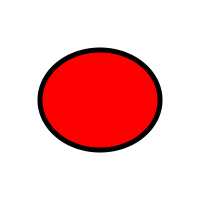
\includegraphics[height=7mm]{img/Icons/Attackers/Red Slime.png}               & \footnotesize{Red Slime}               & 1                   & 5                &                                                                                                                                                             \\
        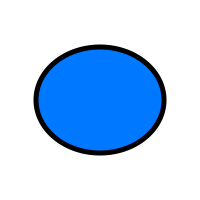
\includegraphics[height=7mm]{img/Icons/Attackers/Blue Slime.png}              & \footnotesize{Blue Slime}              & 1.4                 & 10               & \footnotesize{When killed, spawns a \emph{Red Slime}.}                                                                                                      \\
        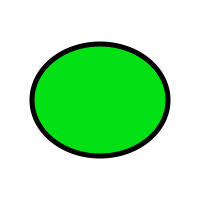
\includegraphics[height=7mm]{img/Icons/Attackers/Green Slime.png}             & \footnotesize{Green Slime}             & 1.8                 & 15               & \footnotesize{When killed, spawns a \emph{Blue Slime}.}                                                                                                     \\
        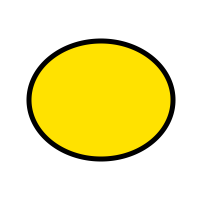
\includegraphics[height=7mm]{img/Icons/Attackers/Yellow Slime.png}            & \footnotesize{Yellow Slime}            & 3.2                 & 20               & \footnotesize{When killed, spawns a \emph{Green Slime}.}                                                                                                    \\
        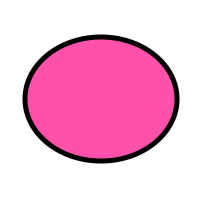
\includegraphics[height=7mm]{img/Icons/Attackers/Pink Slime.png}              & \footnotesize{Pink Slime}              & 3.5                 & 25               & \footnotesize{When killed, spawns a \emph{Yellow Slime}.}                                                                                                   \\
        
\includegraphics[height=7mm]{img/Icons/Attackers/Black Slime.png}             & \footnotesize{Black Slime}             & 1.8                 & 30               & \footnotesize{Immune to \emph{Explosive} damage. \newline When killed, spawns two \emph{Pink Slimes}.}                                                      \\
        
\includegraphics[height=7mm]{img/Icons/Attackers/Lead Slime.png}              & \footnotesize{Lead Slime}              & 1                   & 35               & \footnotesize{Immune to \emph{Physical} damage. \newline When killed, spawns two \emph{Black Slimes}.}                                                      \\
        
\includegraphics[height=7mm]{img/Icons/Attackers/Skeleton.png}                & \footnotesize{Skeleton}                & 1.6                 & 20               &                                                                                                                                                             \\
        
\includegraphics[height=7mm]{img/Icons/Attackers/Yellow Skeleton.png}         & \footnotesize{Yellow Skeleton}         & 1.6                 & 60               &                                                                                                                                                             \\
        
\includegraphics[height=7mm]{img/Icons/Attackers/Black Skeleton.png}          & \footnotesize{Black Skeleton}          & 1.6                 & 180              &                                                                                                                                                             \\
        
\includegraphics[height=7mm]{img/Icons/Attackers/Armored Skeleton.png}        & \footnotesize{Armored Skeleton}        & 0.8                 & 40               & \footnotesize{Has shields that block 1 damage from each hit. \newline Once HP drops below half of max HP, loses the shields and doubles its speed.}         \\
        
\includegraphics[height=7mm]{img/Icons/Attackers/Armored Yellow Skeleton.png} & \footnotesize{Yellow Armored Skeleton} & 0.8                 & 120              & \footnotesize{Has shields that block 3 damage from each hit. \newline Once HP drops below half of max HP, loses the shields and doubles its speed.}         \\
        
\includegraphics[height=7mm]{img/Icons/Attackers/Armored Black Skeleton.png}  & \footnotesize{Black Armored Skeleton}  & 0.8                 & 360              & \footnotesize{Has shields that block 5 damage from each hit. \newline Once HP drops below half of max HP, loses the shields and doubles its speed.}         \\
        
\includegraphics[height=7mm]{img/Icons/Attackers/Big Skull.png}               & \footnotesize{Big Skull}               & 1.2                 & 10               & \footnotesize{\textbf{Large.} \newline When killed, spawns 3 \emph{Skeletons}.}                                                                             \\
        
\includegraphics[height=7mm]{img/Icons/Attackers/Big Yellow Skull.png}        & \footnotesize{Big Yellow Skull}        & 1.2                 & 30               & \footnotesize{\textbf{Large.} \newline When killed, spawns 3 \emph{Yellow Skeletons}.}                                                                      \\
        
\includegraphics[height=7mm]{img/Icons/Attackers/Big Black Skull.png}         & \footnotesize{Big black Skull}         & 1.2                 & 90               & \footnotesize{\textbf{Large.} \newline When killed, spawns 3 \emph{Black Skeletons}.}                                                                       \\
        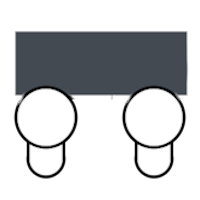
\includegraphics[height=7mm]{img/Icons/Attackers/Coffin.png}                  & \footnotesize{Coffin}                  & 0.4                 & 80               & \footnotesize{\textbf{Large.} \newline Spawns an \emph{Armored Skeleton} every 4s. \newline When killed, spawns 4 \emph{Skeletons}.}                        \\
        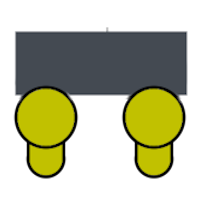
\includegraphics[height=7mm]{img/Icons/Attackers/Yellow Coffin.png}           & \footnotesize{Yellow Coffin}           & 0.4                 & 240              & \footnotesize{\textbf{Large.} \newline Spawns a \emph{Yellow Armored Skeleton} every 5s. \newline When killed, spawns 4 \emph{Yellow Skeletons}.}           \\
        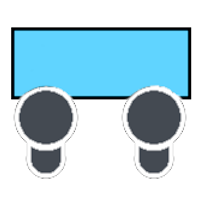
\includegraphics[height=7mm]{img/Icons/Attackers/Black Coffin.png}            & \footnotesize{Black Coffin}            & 0.4                 & 720              & \footnotesize{\textbf{Large.} \newline Spawns a \emph{Black Armored Skeleton} every 6s. \newline When killed, spawns 4 \emph{Black Skeletons}.}             \\
        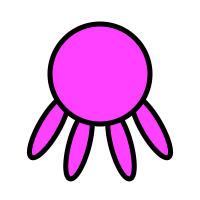
\includegraphics[height=7mm]{img/Icons/Attackers/Jellyfish.png}               & \footnotesize{Space Jellyfish}         & 0.8                 & 8                & \footnotesize{Takes 40\% less \emph{Physical} damage.}                                                                                                      \\
        
\includegraphics[height=7mm]{img/Icons/Attackers/Blue Jellyfish.png}          & \footnotesize{Blue Space Jellyfish}    & 0.8                 & 40               & \footnotesize{Takes 50\% less \emph{Physical} damage.}                                                                                                      \\
        
\includegraphics[height=7mm]{img/Icons/Attackers/Green Jellyfish.png}         & \footnotesize{Green Space Jellyfish}   & 0.8                 & 200              & \footnotesize{Takes 66\% less \emph{Physical} damage.}                                                                                                      \\
        
\includegraphics[height=7mm]{img/Icons/Attackers/Fire Spirit.png}             & \footnotesize{Fire Spirit}             & 3                   & 6                & \footnotesize{Takes 50\% less \emph{Energy} damage.}                                                                                                        \\
        
\includegraphics[height=7mm]{img/Icons/Attackers/Forest Spirit.png}           & \footnotesize{Forest Spirit}           & 2                   & 15               & \footnotesize{Takes 66\% less \emph{Explosive} damage.}                                                                                                     \\
        
\includegraphics[height=7mm]{img/Icons/Attackers/Protector.png}               & \footnotesize{Protector}               & 1.4                 & 100              & \footnotesize{\textbf{Large.} \newline When killed, leaves behind a protective bubble 1.3 tiles in radius that blocks all projectiles from outside for 5s.} \\
        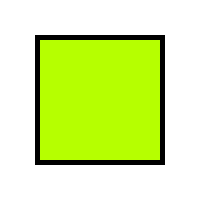
\includegraphics[height=7mm]{img/Icons/Attackers/Druid.png}                   & \footnotesize{Druid}                   & 1                   & 120              & \footnotesize{\textbf{Large.} \newline Every 4s heals each attacker in a 1.6 tile radius by 15 HP.}                                                         \\
        \bottomrule
    \end{tabular}
    \caption{The attacker types in the game.}
    \label{tab:attackers}
\end{table}